\documentclass{IEEEtran}
\usepackage{alphabeta}
\usepackage[euler]{textgreek}
\usepackage[utf8]{inputenc}
\usepackage[english]{babel}
\usepackage{indentfirst}
\usepackage{multicol}
\usepackage{natbib}
\usepackage{amssymb}
\usepackage{hyperref}
\usepackage{amsmath}
\usepackage{listings}
\usepackage{booktabs}
\usepackage{algorithm2e}
\usepackage{bm}
\SetKwInput{KwPre}{Preconditions}

\newcommand{\minuseq}{\mathrel{-}=}
\newcommand{\ubar}[1]{\text{\b{$#1$}}}

\usepackage{multicol}
\usepackage{graphicx}
 
\setlength{\parindent}{2em}
\setlength{\parskip}{0em}
 
\title{Year in industry report}
\author{Mihai Emilian Buduroi}
\date{September 2019}

\usepackage{natbib}
\usepackage{graphicx}

\begin{document}
\begin{titlepage}
\begin{figure}[hbt!]
\centering

\includegraphics{logo_uni}
\end{figure}

\centering

\textsc{\Huge University of Birmingham}\\[0.4cm]
\textsc{\LARGE School of Computer Science}\\[1.5cm]
\textsc{\huge Final Year Project - Project HAWK}\\[2.5cm]
\textsc{\Large Mihai-Emilian Buduroi, 1680948}\\[2.0cm]
\end{titlepage}

\pagebreak

\section*{Abstract} LTE data transfer has come a long way in the past decade. The purpose of this paper is to discuss the advantages and disadvantages of LTE networks in the context of drone control and to illustrate the architecture required for optimizing the communication to the aircraft. To this end, a server-client suite was designed along with the lightweight PCB, housing the array of sensors necessary for stabilization and the computer running on board. The experimental evaluation proved that the main drawback of LTE operability is tower handover when the machine runs at higher altitudes than the ones LTE was designed for. The paper later proposes practical solutions to overcome the impediments revealed by the experiment. What is more, the experimental evaluation also highlights the heat dissipation curve driven by the resistance of the custom PCB in an attempt to maintain safety and reliability.
\section{Introduction}
Cell tower communication is a technology that allows its users to send data over long distances using radio frequencies in the range of 800MHz to 2.4GHz. In the past two decades, this technology has evolved to the point where it allows close to real-time communication between endpoints. The network driven by this technology could be used in controlling unmanned aerial vehicles (UAV), in applications such as transport, reconnaissance and rescue. Due to the vast deployment of LTE networks, this could mean that same-day delivery without employing human resources will soon become available for the general market, and not only for high-end companies such as Amazon \citep{wikipediacontributors_2019_amazon}.
\newline
\newline
This project tests this hypothesis by building a lightweight drone, depending solely on open-source ecosystems such as Raspberry Pi and Linux. However, one potential limitation of the network could be the optimization for ground-level consumers (e.g. pedestrians, cars, houses) and testing this required experimenting the impact of parameters such as RSRQ (reference signal receive quality) when crossing the cell tower signal boundaries at 100m of altitude.
\newline
\newline
This paper will first present the recent technology developments in the field of LTE drone connectivity and their limitations which will be addressed by the current implementation.  Next, the architecture of the system based on a  client-server model communicating using a custom lightweight protocol will be discussed in the light of existent LTE infrastructure. The implementation will then be evaluated in two experiments assessing the LTE connection reliability and efficiency (focusing on towers handover) and the durability of the drone hardware (focusing on heat dissipation over power consumption). Finally, potential solutions for the present limitations and future research avenues will be addressed.
\section{Related work}
\subsection{Parrot Disco UAVPal softmod}
An attempt to enable LTE connectivity in aircraft communication is UAVPal \citep{uavpal_2019_uavpaldisco4g}. The creators introduced an LTE modem and extended the functionality of the software running on the commercial fixed-wing DJI Parrot Disco which was initially designed for running on WiFi. Nevertheless, the prototype uses proprietary architecture, licensing and design. Therefore, it increases the number of dependencies needed and the associated cost, hindering its chances to become a platform that would enable commercial or hobbyist drones to connect through LTE networks. 
\newline
\newline
Moreover, the cited experiment failed to address a problem related to network address translation (NAT), while using a tertiary service to route traffic between the two LTE endpoints. As explained later, this approach introduces latency in propagating the time-sensitive data packets. Other similar experiments faced the same problem due to the lack of hardware/software dependency. This problem was solved by the M2M (machine to machine) network setup which eliminates the various levels of NAT, thus decreasing the time to transmit commands to the drone.
\subsection{Nokia Bell Labs Analysis}
This project partly used an experimental model created at Nokia Bell Labs in Denmark \citep{amorim_2018_measured} which analyses the relationship between received signal quality and latency in non-optimized LTE networks. However, to conduct the experiment the researchers used dedicated equipment to measure the RSRQ. This led to an increased price and the need for highly specialised equipment which is not available for extended production. Given that most robotic equipment production is moving towards affordable technology without sacrificing reliability/performance, the current paper aims to implement a design that minimises cost while maximising efficiency. Thus, instead of recording real-time data during tower handovers, it was based on data from OpenCellid \citep{a2020_opencellid}, removing the need for specialised hardware.
\clearpage

\section{Architecture}
\subsection*{\large{Overview}}
The architecture is based on a client-server model that will communicate using a lightweight TCP/UDP custom protocol over LTE. The server is based on a multi-threaded C application running on Raspberry Pi Zero while the client is based on an Android application. The data that reaches the server is either modifying the virtual state of the drone in the computer or actions or it is encoded and passed further to the pilot. The pilot is a synchronous program running on the 8-bit microcontroller on the PCB and receives data through an analog protocol called PPM.
\subsection*{\large{Background}}
LTE (Long Time Evolution) is a great, easily deployable network technology, which focuses on fulfilling the requirements for the speed and connectivity standards, beginning with 4G. Understanding LTE's limitations and superiority over conventional radio frequency used in drone remote control in the past 20 years, the background of this cellular network technology has to be understood.
\newline
\newline
In the radio-controlled drones world, the range is usually dictated by the reach of the 2.4GHz~2.4835GHz band. Most controller-receiver systems will operate under the range of 150 meters to 1.4 miles (2km)\footnote{DJI Spark can fly as far as 1.4 miles} with exceptions such as the \hyperlink{https://auteldrones.com/products/evo}{Autel Robotics's EVO} which can fly as far as 4.3 miles (7km). All these solutions have a quality in common: they all use private ~2.4GHz point-to-point networks. The reason for this becoming standard is that FCC (or Ofcom for the UK) allowed this spectrum of frequencies for public use  \footnote{\hyperlink{https://transition.fcc.gov/oet/spectrum/table/fcctable.pdf}{FCC Frequency Table rev 2020} page 67} long before the 3G networks or even WiFi were popular.
\subsection*{Pre-digital}
The first generation (or 1G) to be standardized in many countries around the world was introduced in the 1980s and used analog signalling. The transmission speed of this technology was only 2.4Kbps and was only supporting voice. Worse, there was no encryption on the calls, so anyone with a radio scanner could drop in on a call.
\subsection*{Driving the digital cell era}
Starting from 3G, the airtime was split more efficiently (Figure 1): Instead of loading the frequency spectrum, the protocol allocates sequential time slots for each user. Besides this, the protocol is fully digital, which facilitates the IP stack. Then, in March 2009 ITU-R\footnote{International Telecommunications Union-Radio communications sector} specified a set of requirements for 4G standards, the IMT-Advanced specification, requiring 100Mbps\footnote{12.5 MB/s} for high mobility communication (moving cars, trains) and 1Gbps for stationary communication.
\subsection*{LTE and conventional RF}
Summing up this review of the RF space, the main difference between cellular networks and private analog networks lies in the technology and protocols used to transmit data. What is more, The `G` technologies also use cell towers as repeaters to transmit data further. If the towers are abstracted, the private analog network could be compared with FDMA\footnote{Frequency-division multiple access is a channel access method used in some multiple-access protocols.} (Figure 1 b) used to drive 1G in the 1980s. That is, it is an analog signal that can hold up to a number of channels dividing a frequency spectrum.
\begin{center}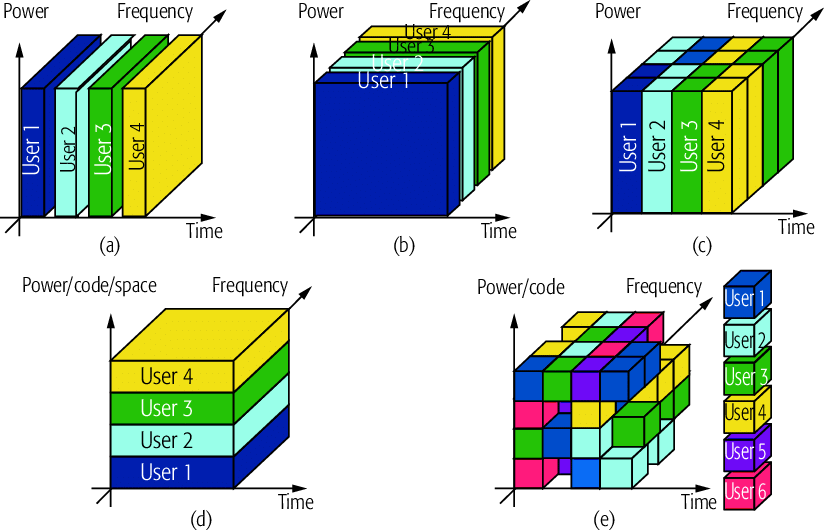
\includegraphics[scale=.3]{FDMA.png}\end{center}
\begin{it}\begin{center}Fig. 1: a) TDMA, b) FDMA, c) OFDMA, d) CDMA/SDMA, e) Possible NoMA Solution \citep{chen_2018_toward} \end{center}\end{it}
\subsection{\large{The server}}
The server is the logical engine for information transmission. In order to achieve all the proposed communication goals (asynchronous internet communication and synchronous PPM), the processor architecture on which the server is going to be run will have to support multi-threading. On top of this, because the application is run remotely, powered by a battery, it also has to be lightweight and efficient. Last but not least, it has to satisfy the connectivity requirements: I2C Bus, USB and direct access to general-purpose  I/O pins (GPIO). 
8
 Therefore, a low-cost portable computer was chosen for the task: Raspberry Pi Zero which only has 9 grams and packs up 512MB of RAM and a single-core 1GHz processor. This connects to three devices (as shown in Figure 2): 
\begin{itemize}
    \item The pilot through a custom PPM\footnote{Pulse Position Modulation} protocol using a GPIO port
    \item A power meter through the Raspberry Pi I2C Bus using the SCL/SDA port
    \item The LTE interface from Huawei (E3372) via USB
\end{itemize}
\begin{center}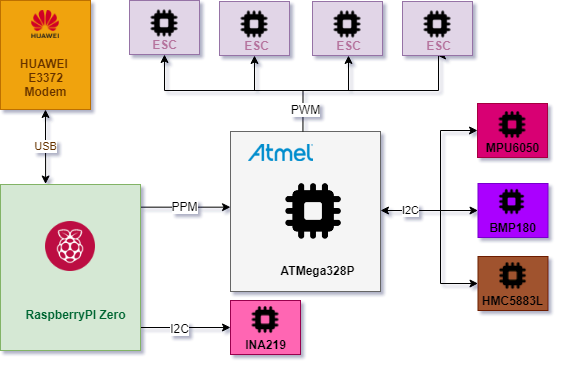
\includegraphics[scale=.45]{server_datapath.png}\end{center}
\begin{it}\begin{center}Fig. 2 - Server datapath \end{center}\end{it}
On the Raspberry, the operating system is a flavour of Linux in the form of Raspbian Lite. Lite was chosen because it comes with little to no bloatware\footnote{Extra apps that might be necessary if one used the Desktop part of the OS, such as Minecraft - Yes, you can play Minecraft on a \$5 PC}.
On the other hand, Linux comes packed with a C compiler (which will be necessary for generating binaries) and the \textbf{glibc} which has implementations for Linux I2C communication, threading, precise hardware timers controllers and sockets. All of the tools are necessary to transform the diagram above into software.
\newline
In the following lines, there will be an explanation about how communication is realized with each of the components in the list above. This will be done from the perspective of the Linux system.
\newline
\subsection*{{1. The PPM Protocol - communicating with the software pilot}}
PPM stands for Pulse-Position Modulation. This protocol is an extension to the PWM (Pulse-Width Modulation) protocol. To understand PPM, PWM needs to be understood first.
\begin{center}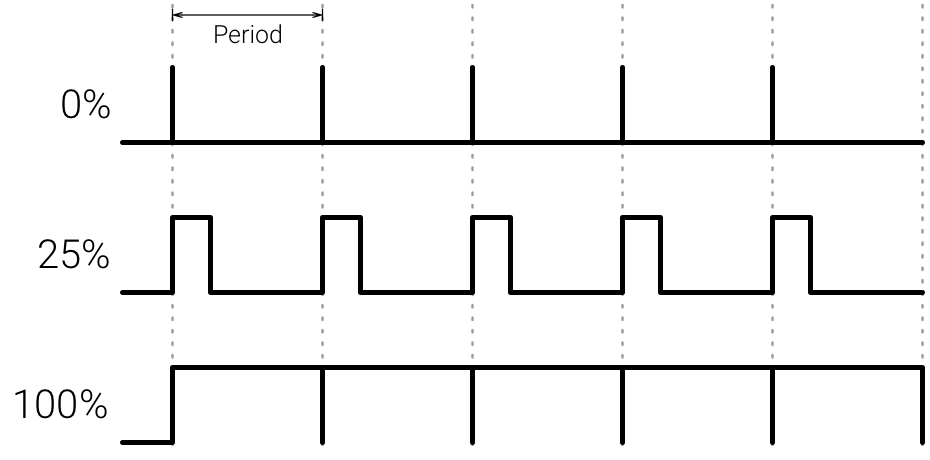
\includegraphics[scale=.24]{pwm-duty.png}\end{center}
\begin{it}\begin{center}Fig. 3 - PWM and duty cycle \end{center}\end{it}
\subsection*{Pulses}
Pulses are a single vibration or short burst of sound, electric current, light, or another wave. Such a pulse can be generated by a relatively simple device. For example, if one was to switch the light on and of in the room and the electrical activity in the circuit was monitored, it would generate a weave that looks like one of the above in Figure 3. 
\newline
\newline
This is exactly what Pulse-Width Modulation is: A way to transmit data at high refresh rates. Looking at Figure 3, The vertical lines represent the switching between ON/OFF. When the value is switched from OFF to ON (from GROUND to positive voltage), the line is called \textbf{rising edge} and the opposite is called \textbf{falling edge}. The \textbf{duty cycle} is the period between the rising edge and the falling edge.
\newline
This protocol is usually used to control servo motors or ESCs \footnote{electronic speed controllers} like this paper is going to showcase later.
\newline
\newline
To sum up, the PWM protocol can transfer information that represents values ranging from 0\% to 100\% duty cycle, but the actual concrete quantities are implementation-specific and depend on the accuracy of the timers used to generate the voltage switches.

\subsection*{PPM - Pulse Position Modulation}
As said earlier, PPM takes PWM and extends it by adding an extra dimension to it. Instead of only using the width of the duty cycle to represent values, it also uses the \textbf{position} (in time). This is useful for storing multiple values in the same wave \textbf{train}. Besides the dimension added, the PPM also adds some complexities. One of them is that the duty cycle is no longer represented by the rising edge - falling edge pair. Instead, consecutive rising edges are used to determine the boundaries of the waves.
\newline
\begin{center}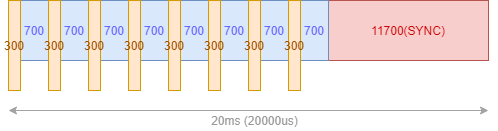
\includegraphics[scale=.5]{ppm2.png}\end{center}
\begin{it}\begin{center}Fig. 4 - PPM theoretical diagram \end{center}\end{it}
In Figure 4 is represented a PPM train (8 PWM pulses linked in a sequence). Each yellow bar represents a period of time in which the switch circuit pulls the signal high. 
\newline
This is how it looks on the oscilloscope: 
\newline
\begin{center}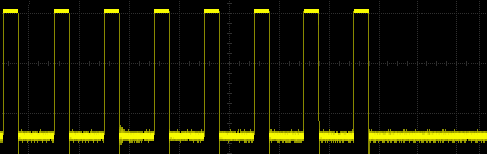
\includegraphics[scale=.5]{ppm.png}\end{center}
\begin{it}\begin{center}Fig. 5 - PPM oscilloscope reading\end{center}\end{it}
When the \textbf{rising edge} is detected (i.e the signal switches from 0 to 5 volts) a logic value is set. This starts a timer that does not stop until the next \textbf{rising edge} is detected. Therefore, if the information in Figure 4 is combined with the information in Figure 5, the following deduction is natural: Each channel represents the arbitrary value 1000 (between each rising edge there is a HIGH signal of 300{\mu}s and a LOW signal of 700). Here is yet another example of arbitrary values to illustrate how the channel values are calculated:
\newline
\begin{center}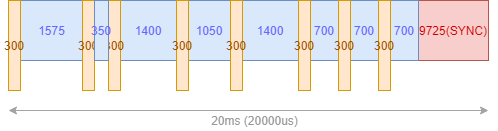
\includegraphics[scale=.5]{ppm3.png}\end{center}
\begin{it}\begin{center}Fig. 6 - PPM practical example\end{center}\end{it}
The following values can be observed:
\begin{multicols}{2}
\begin{itemize}
    \item Channel 1 - 1875
    \item Channel 2 - 650
    \item Channel 3 - 1700
    \item Channel 4 - 1350
    \item Channel 5 - 1700
    \item Channel 6 - 1000
    \item Channel 7 - 1000
    \item Channel 8 - 1000
\end{itemize}
\end{multicols}
The 20ms size for the window is standard in PPM communication. Reducing this is possible only if the timers on the sending/reading devices are precise enough. This will be explored later in this paper.
\subsection*{Synchronization}
To synchronize this signal between the RaspberryPi and the microcontroller, a gap is required (the red portion of Figure 6 and Figure 4). This gap can be observed in all three figures depicted as a long low signal and represents a protocol convention which signals the end of a window and the beginning of another. To be successful, synchronization has to assume three main properties on both systems:
\begin{itemize}
    \item Both of them use the same window size(i.e 20ms or 20000{\mu}s in this case)
    \item The falling edge follows the rising edge after a constant duration
    \item Both systems have timers capable of 1/10{\mu}s accuracy
\end{itemize}

\subsection*{Implementation}
With the theory in mind, implementing this in C depends on the accuracy of the hardware timers. I used a library called \textbf{\hyperlink{http://abyz.me.uk/rpi/pigpio/}{PIGPIO}} that allows the control of GPIO 4 with \textbf{nanosecond} accuracy. This accuracy is better than the requirement for this protocol.
\newline
\newline
There was one remarkable requirement imposed by the library: conserving the signal trains for at least two cycles to achieve synchronisation. That is, it was necessary to wait for two cycles to pass before resetting the memory for the particular train because the hardware requires references to the previous wave when attempting to synchronize. Keeping track of which train was sent was also necessary.
\newline
\newline
The values that were fed to the PPM encoder were served by a structure that, as will be made more clear later, is updated by the network controller.
   
\subsection*{{2. The I2C protocol - communicating to the power meter}}
I2C is also known as a two-wire bus interface. This is a popular digital communication protocol that allows one or more master devices to send and receive data to up to 112 slave devices. In this case, the Raspberry Pi is the master device and the \textbf{INA219} sensor power meter is the slave device. This protocol works using the principle of synchronization. Both devices write and listen to the pulses transmitted through the common line synchronously. The synchronisation is realized by the SCL wire. This is merely a constant alternating pulse between GROUND and signal voltage (3.3V in this case). The SDA wire is the medium that transfers digital information. 
\begin{center}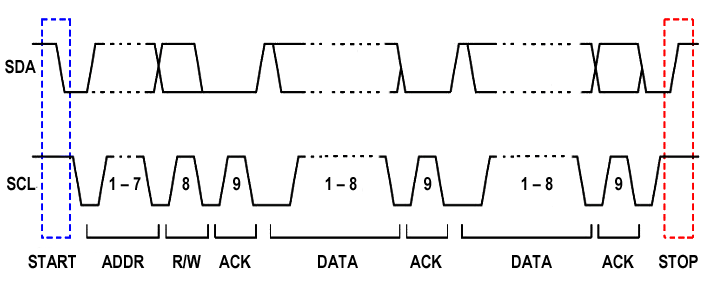
\includegraphics[scale=.35]{i2c.png}\end{center}
\begin{it}\begin{center}Fig. 7 - Generic i2c message \end{center}\end{it}
This follows a robust protocol as shown in Figure 7:
\begin{itemize}
    \item The master initiates a START condition
    \item The master sends a 7-bit address of the device and a bit representing the intention for WRITE
    \item The slave responds with an ACK/NACK condition\footnote{ACK response is when a machine confirms success on receiving data}
    \item On ACK, the master sends the register it intends to write to and the device will store this address for later use.
    \item The slave responds with an ACK/NACK condition
    \item On ACK, the master can continue by either sending a byte of data to change the contents of the register in step 4 or re-initiate the START condition and send the address of the device followed by a READ bit to read data.
\end{itemize}


\subsection*{Implementation}
The hardware requirement for this protocol to work properly is that both the voltage powering the sensor and the voltage on the SDA/SCL lines were equal. Also, the pull-up resistors values have to be carefully considered, but in this context, the Raspberry Pi fulfils both requirements. An example where pull up resistors had to be chosen manually will be presented later in this paper. What is more, the interaction with the i2c bus was made possible using the character device API \textit{linux/i2c\_dev}. This library supports all the steps described above and in Figure 7.
\newline
\newline
Furthermore, reading and writing are required to use the sensor at maximum potential. The read values are used to update the global \textbf{drone\_state} structure which holds variables for voltage, current and power.
\newline
\newline
Last but not least, to sample the correct information from the power meter sensor, two registers have to be set up: Configuration Register and Calibration Register. The first registers will set parameters such as sampling type, max voltage, sampling resolution etc. For this project the maximum voltage was set at 16, the sampling type was set on "averaging" (great for determining battery voltages) and the maximum resolution was used. The calibration register sets the maximum expected current and the shunt resistor value which will impact the samples of the sensor by scaling the data register values (register map covered in section 8.6 of the datasheet). Setting up this register is covered in the datasheet in section 8.5.1
\subsection*{{3. The HAWK 1.0 Protocol - communicating to the internet}}
\subsection*{Development reasons}
\noindent Communicating to the drone via LTE broadband brought up a set of requirements for the protocol:
\begin{itemize}
    \item Be reliable when sending critical commands such as ARM / DISARM / LAND / FLIGHTMODE
    \item Be fast when sending stick movement commands (axes update)
    \item Be lightweight and robust to keep bit rate low
\end{itemize}
None of the available protocols was satisfying all the requirements so this had to be engineered around the reliability of TCP and the speed of UDP. For this reason, the HAWK 1.0 protocol was based on both TCP and UDP to transmit information. The information is transported from the Android client to the C server and back. This means that both ends can generate and read this protocol.
\newline
\newline
\noindent Assuming 60 bytes (maximum) for the TCP header and a number of N=5 values in the parameters list, the packet size would be 126 bytes\footnote{41 bytes (from the header) 25 bytes from parameters and 60 bytes from the TCP header}. Figure 8 describes all the field sizes and their order.
\begin{center}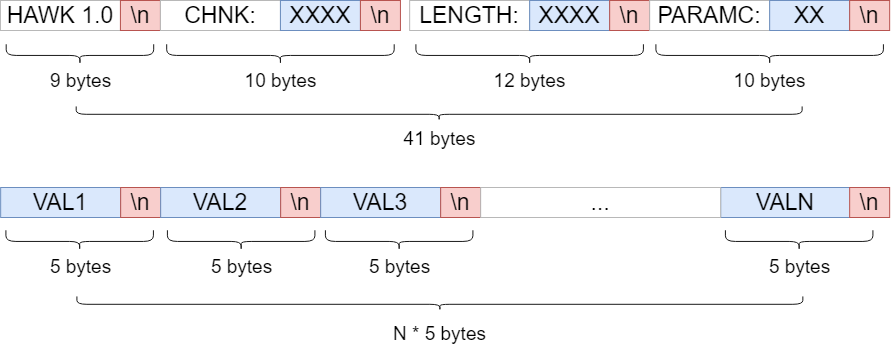
\includegraphics[scale=.29]{hawkone.png}\end{center}
\begin{it}\begin{center}Fig. 8 - HAWK 1.0 structure \end{center}\end{it}
\subsection*{Implementation}
Implementing this protocol and making it work is one of the bigger pieces of development in this project. The protocol is bidirectional which means that each end (client and server) must be able to both send and receive messages of this type. The messages are sent \textbf{asynchronously} which means that at any time packets might be in air\footnote{Generated and sent, but not yet arrived at destination}. The full potential of the Raspberry Pi and Linux environment is shown with this part of the project. 
\newline
\newline
Because multi-threading is supported on the ARM11 SoC \footnote{ARM architecture system-on-chip, packaged by Broadcom in BCM2835}, running asynchronous processes in Linux is as easy as calling \textit{pthread\_create()}. This is in fact what was done in this case - threads were invoked for:
\begin{itemize}
    \item listening for UDP packets
    \item listening for TCP packets
    \item sending TCP packets
\end{itemize}

\subsection*{TCP and state control}
The UDP stream is dependant on the TCP connection. The state machine that drove the development is depicted in Figure 9.
\begin{center}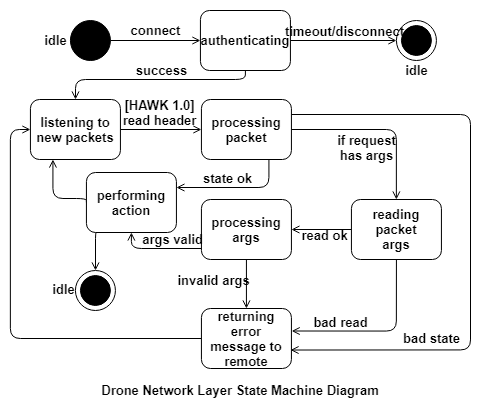
\includegraphics[scale=.45]{net_state_machine.png}\end{center}
\begin{it}\begin{center}Fig. 9 - Network Manager - State Machine Diagram \end{center}\end{it}
The TCP connection is controlling the state of the system in multiple ways. For example, when the program is launched, the UDP listener is blocked in a sleeping loop until a message to change the state is received through TCP. Another example of state change is inherent from the presence of a connection: The system only allows for one connection to exist at a time, therefore when a second client attempts to connect, the socket revokes the request.
\newline
\newline
Another potential implementation of the state machine presented above uses TCP only. Nevertheless, ACKs would double the latency of the remote and cause potential retransmissions, resulting in further delays of the packets. Therefore, UDP  and its ”send and forget” policy represents a better choice for the current implementation due to time saved in not checking whether the target received the data.
\subsection*{{3.1 The LTE modem}}
The LTE modem is one of the core components for running this project, being second only to the ARM SoC on the Raspberry Pi.
\newline
This, together with a custom SIM card are the components that have allowed the project to be accessed from the public internet. The key difference between consumer SIM cards and the one used for this project is CGNAT or Carrier Grade Network Address Translation. This means that the IPS\footnote{Internet Provider Service} and suppliers, to offer all customers a fair share of the IPv4 range of IPs (4,294,967,296 or $2^{32}$) which is close to exhaustion, need to insert a new dimension of complexity: private IP multiplexing. This means that each client is sharing a pool of public IPs reserved by the provider. The network address translation is done by the routing hardware, thus enabling private IPs. However, the private IP is only known by the provider and, reaching a machine hosting a server from public internet is not directly possible. By \textit{"not directly"} is meant that there are alternate ways to make the machine-accessible from outside and here are a few solutions tried:
\begin{itemize}
    \item Use a VPN - Meeting with the client in the middle, on a third station would allow to create a hole in the internet and allow packet exchange freely
    \item Use reverse SSH - two machines connected to an SSH server can cross-communicate.
    \item Use a base station server - The server is hosted on the ground and all packets are forwarded between client-drone and client-remote.
\end{itemize}
As it can be observed, all the items above involve some sort of packet routing through a third component. This is a major overhead when working with under 50ms latency systems. If the average ping time \footnote{the time it takes to send 1 packet or 1/2 Round Trip Time (RTT)} from Birmingham to London is 25ms, it would be fine to route the packets through a ground station in London to communicate to a drone in Canterbury. However, once the packet target is moving West or, even if it is local to Birmingham, several milliseconds of latency are added. For example, the median latency from Birmingham to Dublin is 38ms. Routing packets through London would add an overhead of RTT Birmingham to London which is 50ms, summing up to 88ms theoretically. In practice, the tolerances are much worse and they will be explored during experimental evaluation.

\subsection*{Configuring the LTE Modem}
The modems available on the market are factory configured with commercial use in mind. The chipset supports two main modes of operation: MODEM MODE and STICK MODE
\newline 
\newline
MODEM MODE (which is factory default) allows users to connect to the stick in two ways: either through the USB interface or through a hosted hotspot. Accomplishing this type of connectivity requires a layer of network address translation. That is, packets arriving from the public internet would be routed to the specific IP addresses generated by the local DHCP server inside the modem. This is yet another overhead, just like previously when the NAT was done by the network provider. This problem can be usually solved by using port forwarding. This, however, is not available on this particular modem and, therefore, an alternative solution is using stick mode.
\newline
\newline
STICK MODE is a mode of operation for the Huawei LTE modem that allows 1 to 1 connectivity with the public internet. Now the device is fully open to the public internet which means that all the services hosted on the Raspberry can now be accessed from anywhere in the world. Potential security risks are mitigated by securing the  SSH  server with a  public/private key pair  (instead of the usual password) and firewall policies.
\subsection*{Enabling STICK MODE}
The steps outlined below are derived from the datasheet of the microprocessor and require cloning forth32/balongflash and forth32/balong-usbdload. It requires cloning \hyperlink{https://github.com/forth32/balongflash}{forth32/balongflash} and \hyperlink{https://github.com/forth32/balong-usbdload}{forth32/balong-usbdload}:
\begin{itemize}
    \item[] 1. Pry open the modem case and using two probes linked by a wire, short the test point pad to Ground
    \item[] 2. Connect the grounded modem to a Linux machine. Now powered up, the modem will have launched in a special bootloader mode. 
    \item[] 3. usbdload linked above is used to put the stick in a non-persistent download mode.
    \item[] 4. balongflash could then be used to flash the firmware available in the second repository
\end{itemize}
\clearpage
\pagebreak
\subsection{\large{The client and the remote}}
The client is an Android application which interacts with the server by using the HAWK 1.0 protocol explained in a previous section; capable of sending and receiving TCP packets from the server. As explained before, sending TCP packets is useful for ensuring critical requests are received by the drone. The inbound TCP packets are not critical to the functionality of the drone, but they are useful for receiving information about power consumption, battery level and crash status.
\newline
\newline
The application is built using the MVC pattern (Model View Controller - Figure 10)).
\begin{center}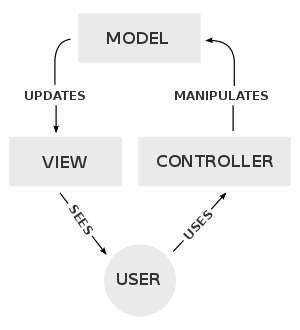
\includegraphics[scale=.35]{mvc_pattern.png}\end{center} 
\begin{it}\begin{center}Fig. 10 - MVC pattern \end{center}\end{it}
\subsection*{{1. The View}}
\noindent The view is composed of three main screens. In android, these screens are called activities. The purpose of the\textit{Splash Activity} is presenting the application to the user and hides the application until all facilities are loaded (ping check to the drone IP, ping check to the public internet, battery percentage).
\begin{center}
\includegraphics[scale=.4]{splashscreen.png}\end{center}
\begin{it}\begin{center}Fig. 11 - Splash Screen Activity \end{center}\end{it}
. This activity lasts for about 900 milliseconds, depending on the signal strength, and the user cannot interact with it.
\newline
\newline
The main activity is the virtual place where the user will spend the most time. It has four visible elements forming a dashboard (as seen in Figure 12). Controlling the drone is only possible in this activity.
\begin{center}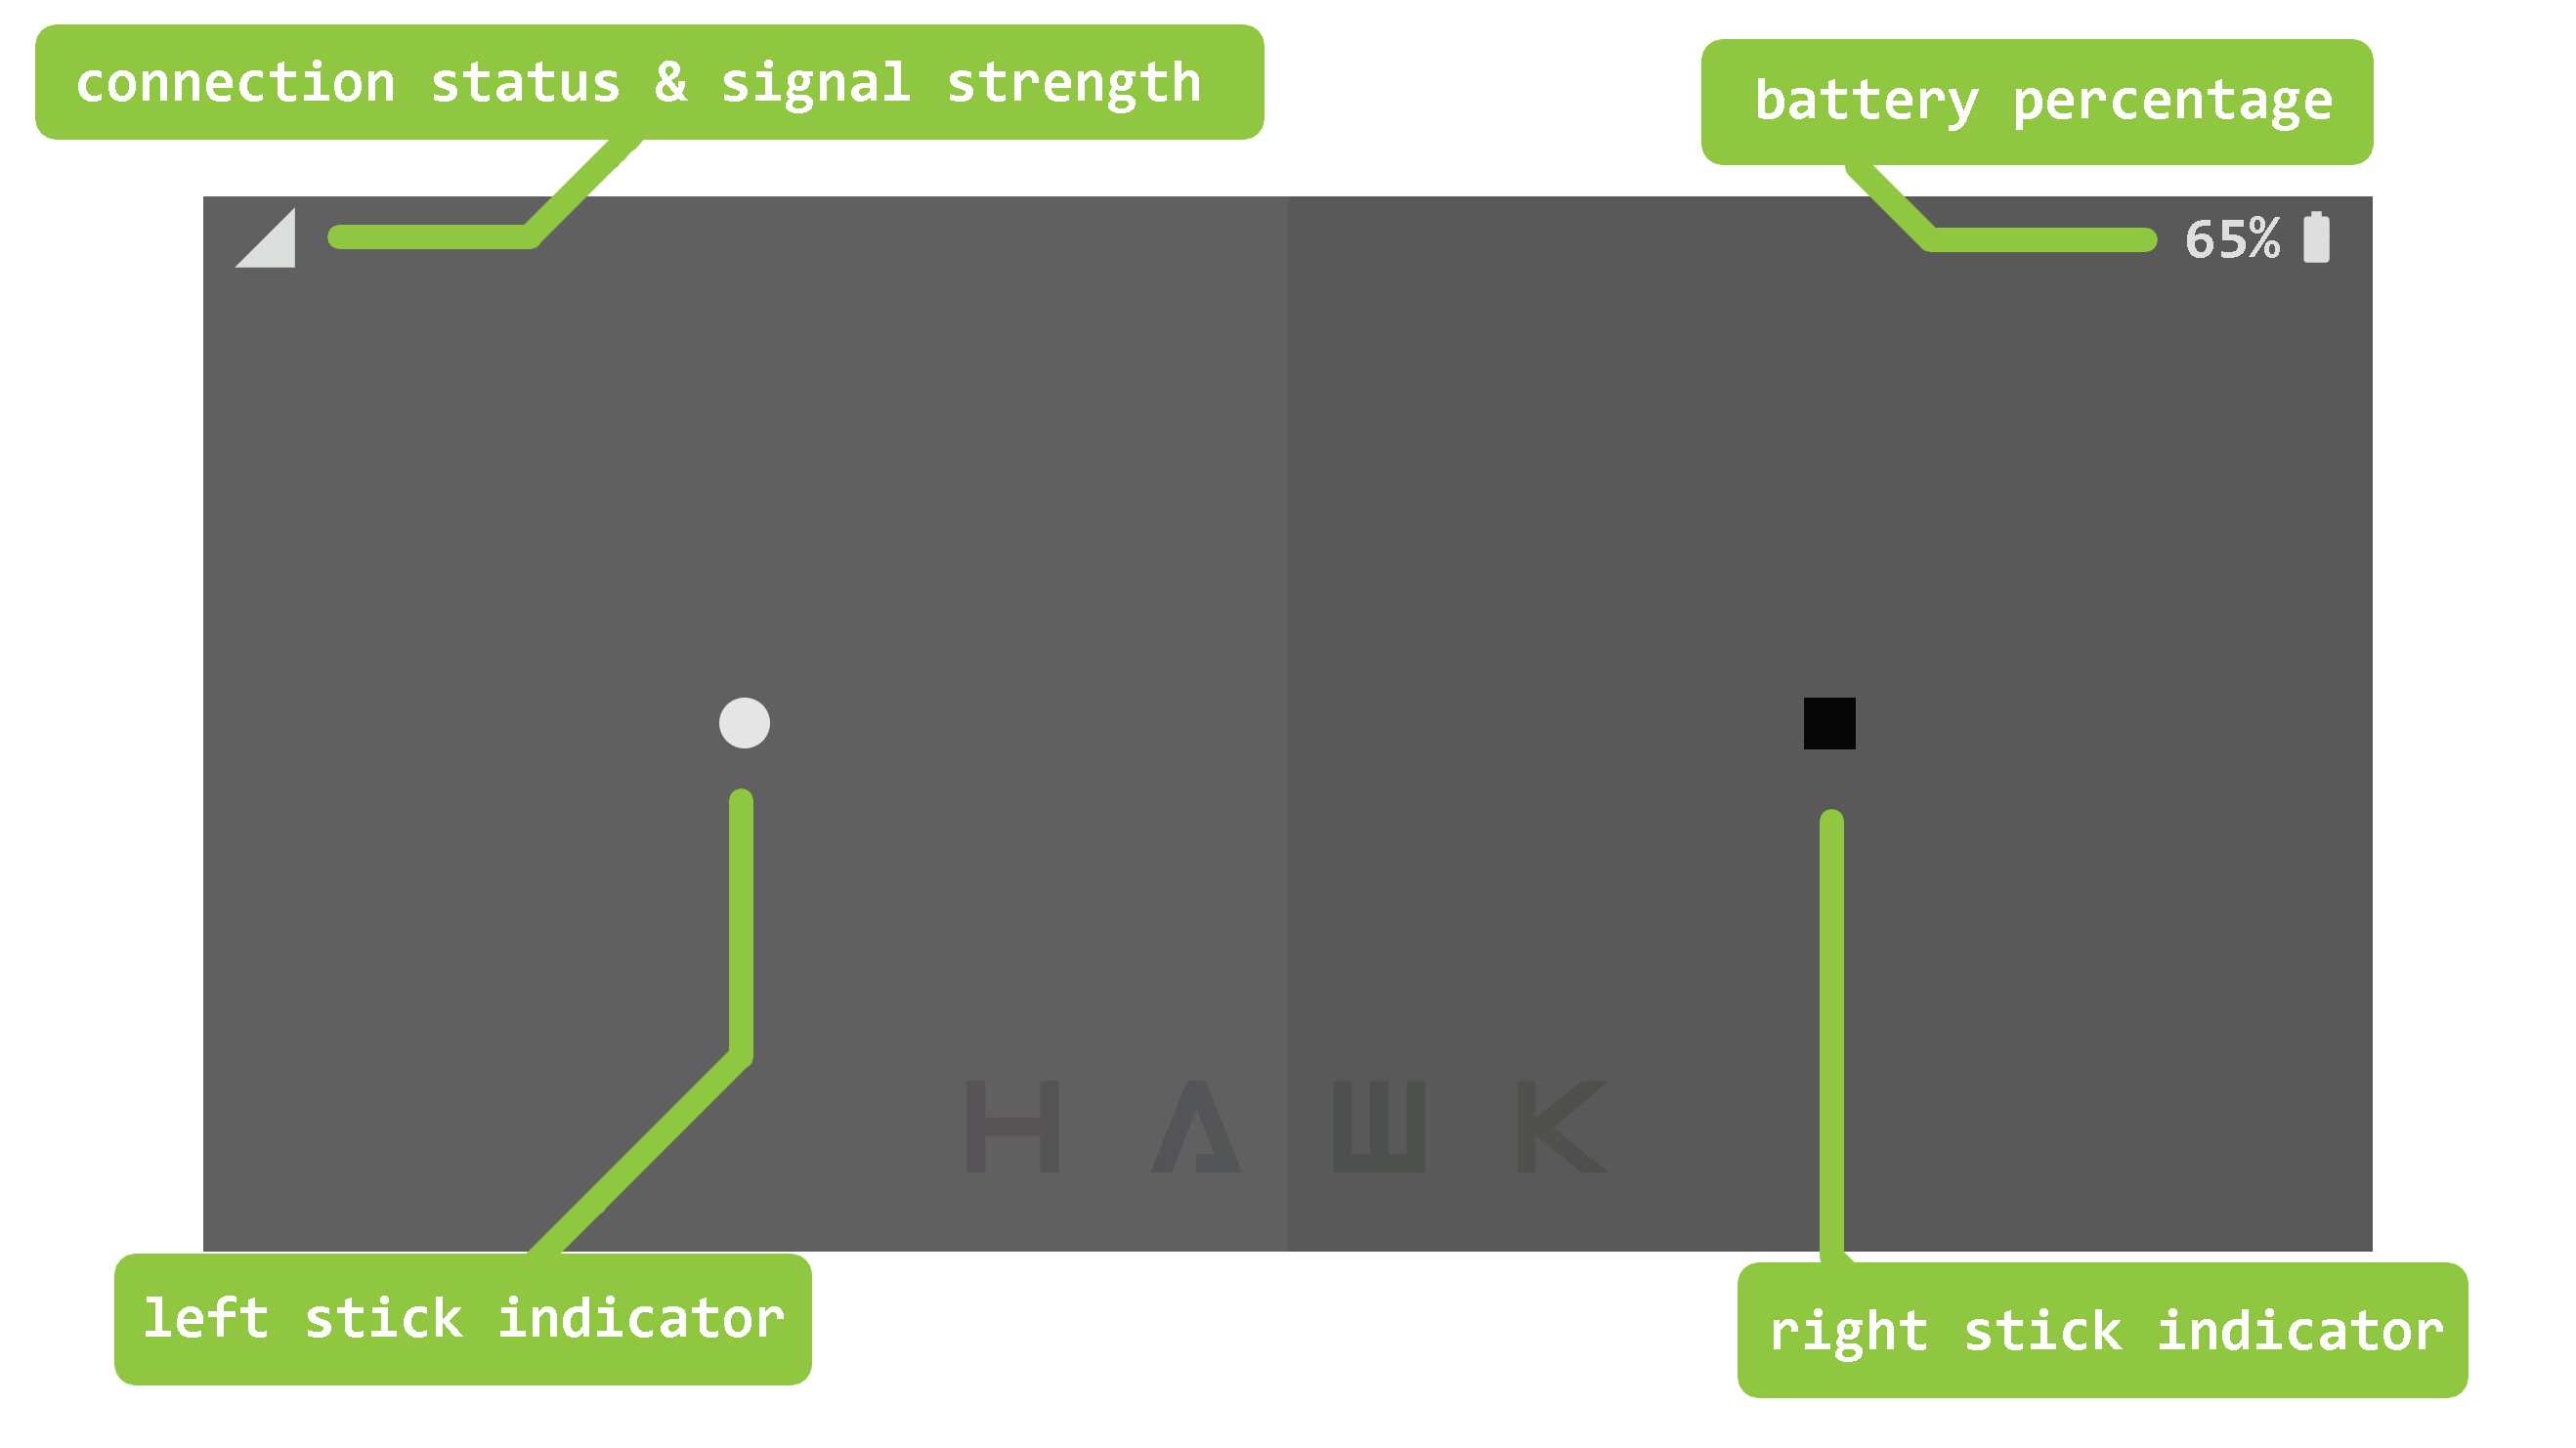
\includegraphics[scale=.10]{remote1.png}\end{center}
\begin{it}\begin{center}Fig. 12 - Main activity \end{center}\end{it}
The last activity is a settings panel which can be accessed pressing a button on the remote (see Figure 13). The settings are preserved in the app globally using the android API -  \textit{SharedPreferences}. This allows to save the values for settings like \textbf{Drone IP}, \textbf{Flight Mode} and  \textbf{Telemetry switch}.

\begin{center}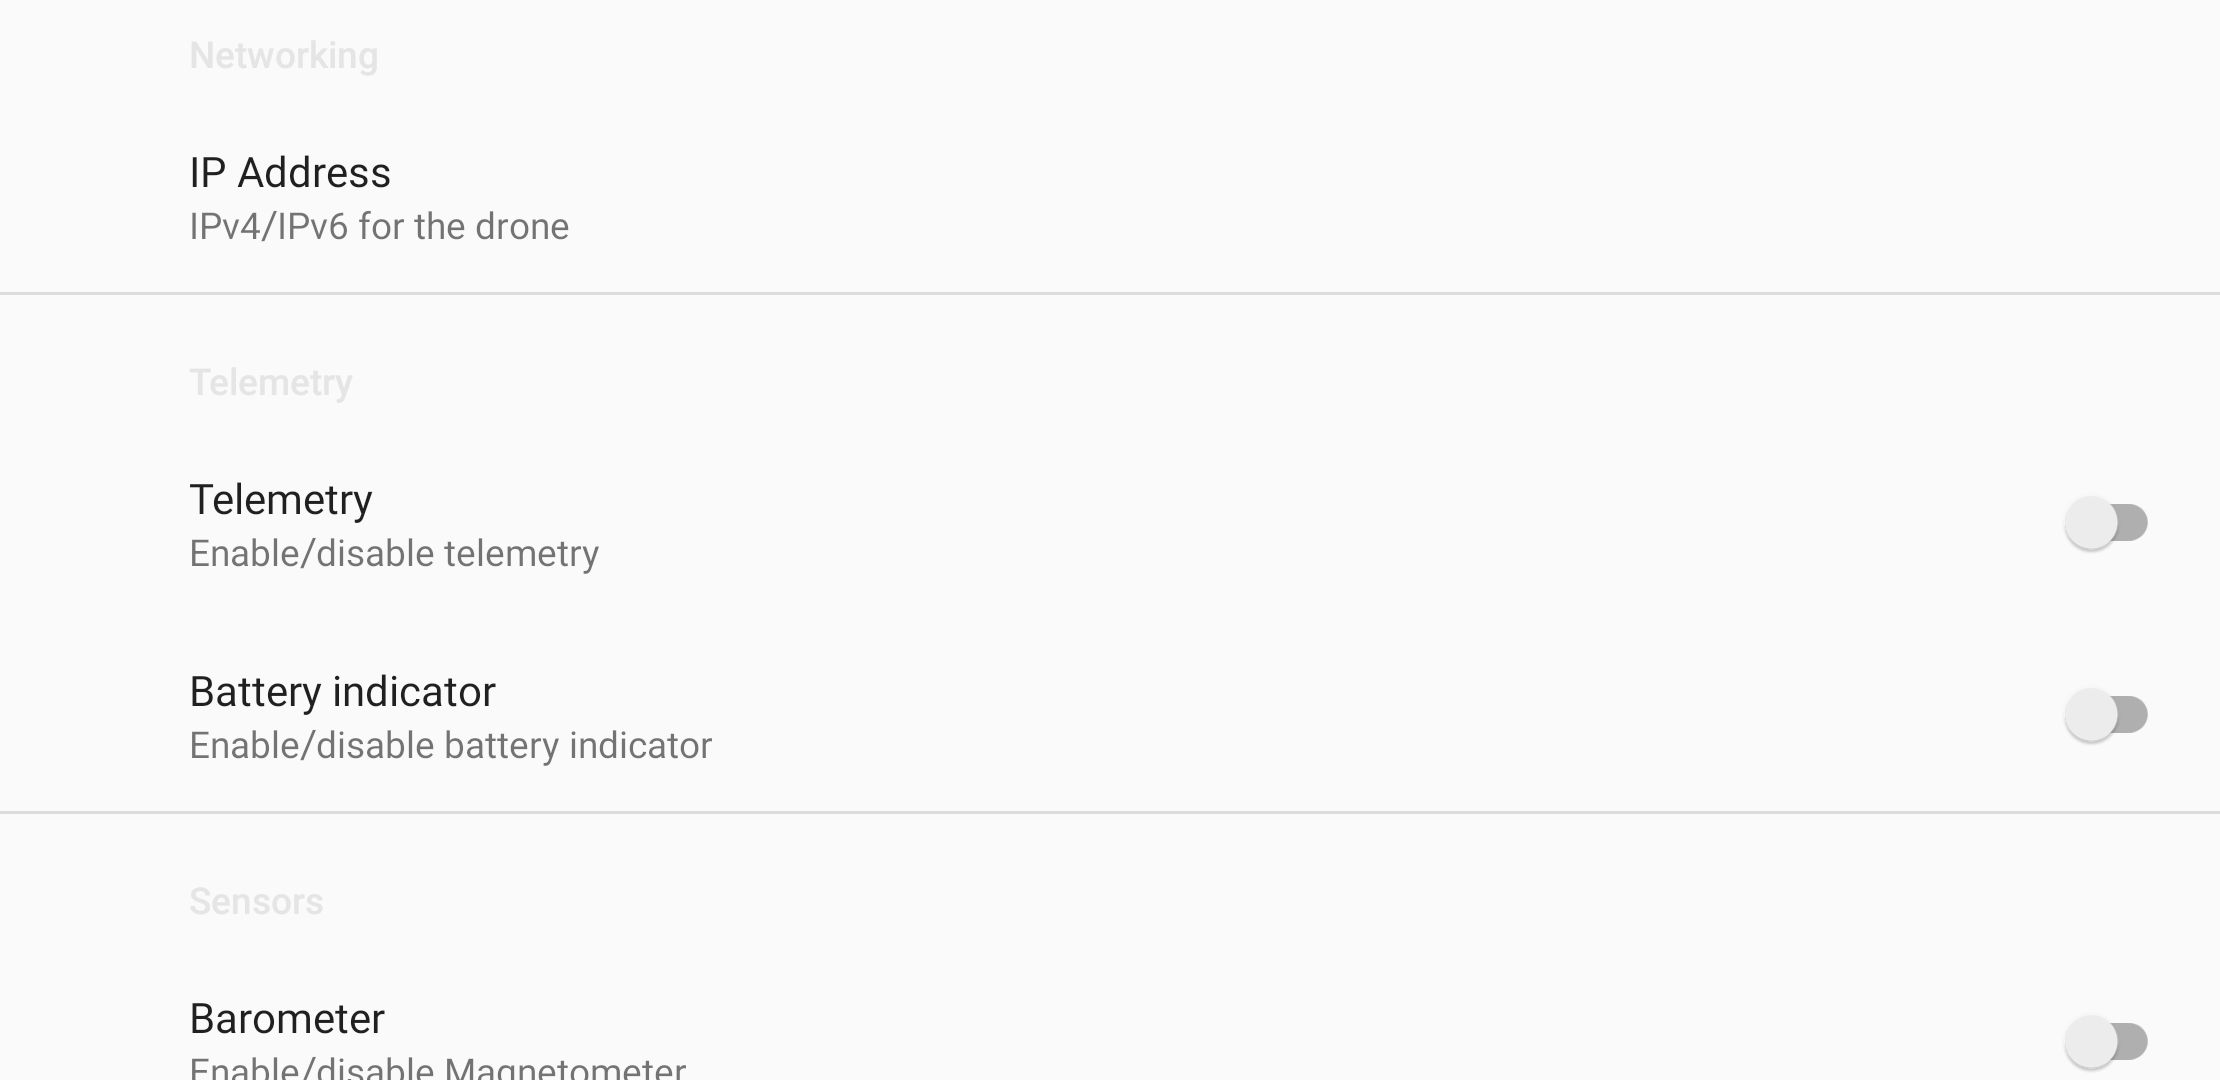
\includegraphics[scale=.11]{sharedpreferences.jpg}\end{center}
\begin{it}\begin{center}Fig. 13 - Settings activity \end{center}\end{it}

\subsection*{{2. The Controller}}
\noindent In this application, the controller interacts with both the user and the drone (through the network). Interacting with the user, it passes data from the model to the view and, reversely, from the remote and the touch screen interface to the model. When it interacts with the drone it passes the commands from the model to the drone and back.
\newline
\newline
The controller is responsible for all the communication on the client-side. This is achieved by running parallel threads and services. For sending and receiving TCP messages with the HAWK 1.0 protocol, \textit{AsyncTask} is used to run two independent threads. These are executed from a thread pool. This allows the user to start and stop the threads at any time (i.e stop the communication to the drone and return it). 
\newline 
\newline
Sending UDP packets to the server, however, was more difficult to do with accurate timing. Android devices, although powerful, are built upon embedded architecture. This architecture has been created with the RIS pattern in mind (Reduced instruction set), thus giving it the name RISC (RIS Computer). This means that, at the processor level, complex tasks are completed using small simple steps. One complex task is process scheduling. This allows a computer to parallelize tasks and create contexts based on those. For example, when one uses the command "sleep(\textit{t})" in a process, the processor knows that the machine and user would benefit from performing a different task.  Switching between two tasks is named accordingly, "\textit{context switch}"
\subtitle{Context switches are expensive}
When interacting with remote devices at under 50ms latency, time is crucial. Just like in this application, the time between two subsequent packets has to be minimized. This can be accomplished by sending many packets per second at fixed intervals. The Android API supports JAVA's \textit{nanosleep(t)} and \textit{microsleep(t)} functions. One naive approach would be to start an Asynchronous task (thread in android) and \textit{microsleep(t)} for t amount of time. This would mean that if one wanted to implement a thread that executes a job 500 times per second, they would have to use \textit{microsleep(20000)} in a loop that contains the task. However, in Android, a context switch is very expensive (20 milliseconds). That means that any amount of time used in a \textit{sleep(t)} function would make the processor take at least 20 milliseconds to return to the task. This limits the frequency of a job to 50 times per second (in theory) and in this context artificially adding 20ms to the system is not acceptable.
\newline
\newline
One solution is developed by the Oracle engineers: \textbf{ScheduledExecutorService}. ExecutorService is a framework provided by the JDK\footnote{Java Development Kit} which simplifies the execution of tasks in asynchronous mode. What is more, this also allows for the execution of tasks at fixed intervals, which is precisely what the requirement is for the UDP packet sender. With this framework, the client can send up to 4000 packets/second. In practice, 250 messages per second will decrease the delay between packets down to 4 milliseconds, which is the way it is implemented in this project. 
\newline
\newline
The controller is regulated by a set of states stored in the model. All the threads follow this sequence: They are created at the beginning and run in loops that allow them to sleep indefinitely until the user requests to connect to the drone. Once the socket connection is completed, a state change is noted and they operate in their main use case scenario. When the user disconnects, all threads return to sleeping. Finally, when the user exits the app, the threads are returned to the thread pool.
\newline
\newline
The TCP sender follows the generator-consumer principle. When the user presses a button that is linked to a request (land/arm/disarm), a packet is generated and added to a blocking queue. The TCP sender then removes the packet from the queue and sends it to the server.
\newline
\newline
On the other hand, the UDP sender has a different approach. If the remote is armed, the UDP sender reads the current state of the joysticks (all 6 axes + 2 extra) and sends it continuously, 250 times per second. The packets change only when the user moves the joysticks. This facilitates a great response time and the network will also respond by offering the best route for the packets to reach the server.


\noindent The connection status is set by the controller and it is managed by the \textit{TCPSender} thread. The controller also manages the battery percentage indicator by using the energetic model provided by the manufacturer in the datasheet (i.e the server sends the voltage of the battery and this is transformed in battery percentage)
\newline
In this activity, the connected Bluetooth gamepad is the most important user input interface. Below is a map of commands.
\begin{center}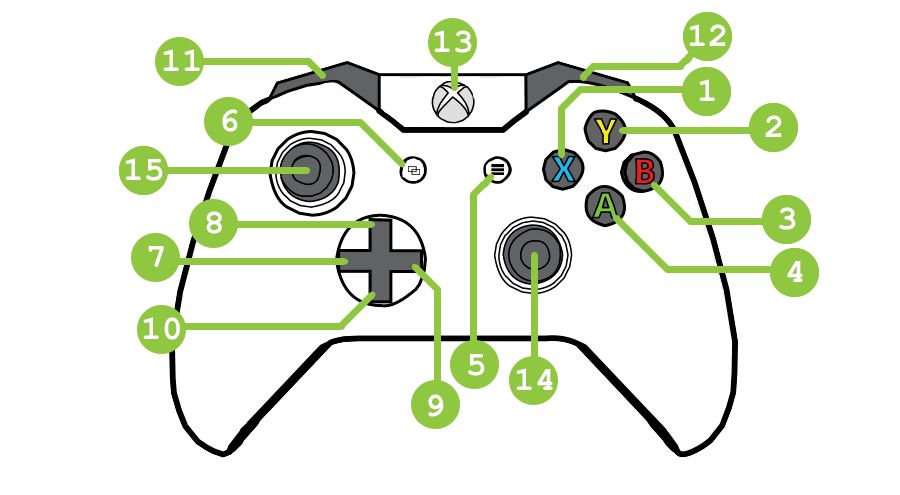
\includegraphics[scale=.3]{gamepad2.png}\end{center}
\begin{it}\begin{center}Fig. 14 - Controller commands map \end{center}\end{it}
\begin{multicols}{2}
\begin{itemize}
    \item[] 1. Toggle battery reading
    \item[] 2. Toggle telemetry
    \item[] 3. Disarm remote
    \item[] 4. Arm remote
    \item[] 5. Enter menu activity
    \item[] 6. Pilot arm switch
    \item[] 7. - throttle gain
    \item[] 8. - base throttle
    \item[] 9. + throttle gain
    \item[] 10. + base throttle
    \item[] 11. - pitch/roll gain
    \item[] 12. + pitch/roll gain
    \item[] 13. Connect to drone
    \item[] 14. Altitude hold 1
    \item[] 15. Altitude hold 2
\end{itemize}
\end{multicols}

Here's an explanation for some of the functions listed above:
Pressing button tagged \textbf{13} will attempt to connect to the server hosted on the drone. On success, the signal status will change into white and it will display the signal strength. On failure, it will become red.
\newline
Once connected to the drone, the user can request telemetry data such as battery voltage (which the model will convert into battery percentage) and flight status (i.e crashed/landing/armed/disarmed) by pressing buttons tagged with \textbf{1} and \textbf{2} respectively.
\newline
\newline
Starting the drone for flight has two phases: a) arming the remote (pressing button \textbf{3}) and b) arming the pilot. Arming the pilot is made in a sequence to avoid unintended commands. This command will start the motors and the drone becomes operational. To arm, the pilot the user has to press and hold button tagged \textbf{6} and push the right stick (Figure 15) up (+YR). Disarming the pilot has a similar sequence, but the stick has to go down (-YR).
\newline
\newline
Once the drone is in the air, if the buttons \textbf{14} and \textbf{15} are pressed, the drone will hold altitude. This can be cancelled by pressing either of buttons. The drone can be landed either manually or automatically by pressing button \textbf{2}.
\newline
\newline
The position and orientation of the drone can be modified using the joysticks in Figure 15 as follows:

\begin{center}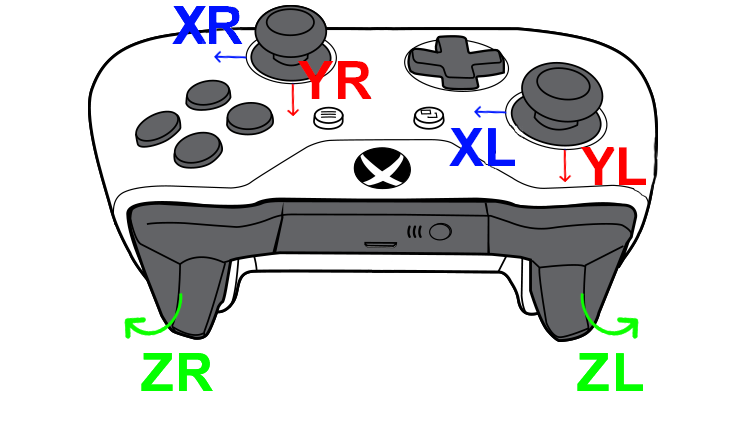
\includegraphics[scale=.35]{gamepad1.png}\end{center}
\begin{it}\begin{center}Fig. 15 - Controller axes \end{center}\end{it}
\begin{itemize}
    \item[] a. Right stick axis (XR) will control the YAW of the aircraft (the orientation or rotation on the horizontal plane
    \item[] b. Left stick axis (XL) will control the ROLL of the aircraft (the inclination towards left or right)
    \item[] c. Left stick axis (XR) will control the PITCH of the aircraft
    \item[] d. Right shoulder pad (ZR) will increase the throttle, thus making the drone lift
    \item[] e. Left shoulder pad (ZL) will decrease the throttle, thus making the drone decline
\end{itemize}

\noindent The Xbox One gamepad is directly managed by the controller by using a set of listeners for button presses, axes movement and special sequences. Unlike the threads that run the networking tasks, this part of the controller operates on the UI thread like the rest of the switches and buttons in the View.
\subsection*{{3. The Model}}
\noindent The model comprises all the static data stored in the SharedPreferences, the RemoteState object and all the functions associated with saving and retrieving data from those. This also includes all the functions that transform the data passed from the user by the controller. Also, there is a class called Packetizer which, as its name suggests, packages information into packets for outbound for both UDP and TCP traffic. Depending on the type of packet, the Packetizer will either pack data continuously from RemoteState variables (in the case of UDP packets) or upon request from the Controller (for TCP packets). Last but not least, the model implements an array of functions which translate the user input depending on the level of experience the pilot has set in the application. For example, a novice pilot can have joysticks that impact the yaw, pitch and throttle less aggressively. 
\subsection*{Shared Preferences}
\noindent As with the android API, the SharedPreferences framework is a great tool to save data in files managed by the android OS. In this project, this was integrated using a PreferencesFragment instance (extended by the MenuFragment class). What it does is to set the preferences from an XML resource managed by the application and recognized by the OS. Thus, all the settings are preserved between sessions.

\subsection*{RemoteState}
\noindent RemoteState is a class that, when instantiated, it creates all the necessary objects, variables and arrays to store all the necessary data for determining the state of the client. This includes:
\begin{itemize}
    \item Button states on the remote (pressed/not pressed/pressed how long ago)
    \item Connection status
    \item Joysticks and shoulder pad position - all 6 axes are stored in an array
    \item Battery status when read from the drone
    \item Crash status when sent by the drone
    \item Arming status
    \item All virtual states such as pilot level, active telemetry, flight mode etc
\end{itemize}
Finally, combined with the settings activity, the remote state provides a great platform for managing the list of parameters used by the pilot during flight. 
\newline
\newline
Wrapping this section up, the Model View Controller pattern was used due to its high modularity which allows the developer to customize features as requirements change without creating a strong dependency between its components.

\clearpage
\pagebreak
\subsection{\large{The PCB and pilot}}
\noindent There were three goals that were set when planned building a custom PCB. The main goal was to reduce the overall weight of the drone by reducing the number of cables and circuitry. The board weighs 28 grams (including all the components and the Raspberry Pi Zero, that is 17 grams empty) - compared to the initial prototype which weighted 210 grams in cables (including power lines and jumper cables), components and structure plate.
\newline
\newline
The secondary goal was to offer mechanical structure and strength for the body of the drone. The board has sixteen mounting holes that allow to securely mount the four arms. At 1.6mm thickness, the fibreglass (Which is the main material) offers flexibility to the PCB, while the copper layers offer rigidity. Together, the PCB is a flexible and lightweight, yet strong plate which has proven to last long during high-speed crashes and drops from the sky. 
\newline
\newline
The final goal of the PCB was to offer circuitry reliability and neatness to the project. The main flying prototype for this project was built using jumper cables and external power wires\footnote{\hyperlink{https://www.youtube.com/watch?v=LCkdW5JWxsk&feature=youtu.be}{Here's a link to the first flying prototype}}. The PCB has two layers of copper and the design separates the logical wiring from the power distribution.

\subsection*{The design}
\noindent The design emerged straight from requirements: One flat panel that could easily and cleanly house an array of sensors required by the pilot, which could be connected to the Raspberry Pi Zero.
\newline
\newline
The design of the PCB started with dividing the necessary components into three categories or three logical blocks: The microcontroller, the sensors, and the power distribution system. From each block, a schematic emerged.
\begin{itemize}
    \item Microcontroller schematic - Appendix 1 
    \item Inertial Measurement Unit Schematic - Appendix 2
    \item Power Distribution Schematic - Appendix 3
\end{itemize}
The first block is comprised of all components that are closely related to the microcontroller. The microcontroller does not have an internal oscillator, thus, an external oscillator is required. A 16MHz oscillator is recommended by the datasheet of the microcontroller (\textbf{ATM\_OSC}). The two capacitors required for the oscillator have been integrated with the oscillator chip. Other passive components such as capacitors ensure voltage filtering (ATM\_C1, ATM\_C2, ATM\_C3, ATM\_C4) and pull up resistors which rectify the i2c bus's reference signal when the gates inside the masters and slaves close. The logic states are represented by two voltage levels, with any voltage bellow one level regarded as logic "0" and any voltage above another level regarded as logic "1". In this case, the devices interpret values in the range 0-3.3V with voltages over 2.8V as logic "1" and bellow 1.6V as logic "0".  Not using the mentioned resistors could lead to a voltage level between 1.6V and 2.8V, introducing errors in the protocol.
\subsection*{The pilot}
The stabilization software was chosen in pair with the microcontroller that runs it. The software is called MultiWii 2.4 \citep{a2020_multiwii} and it runs on a small set of 8-bit microcontrollers. This is an earlier version of BetaFlight \citep{betaflight_2020_betaflightbetaflight} which grew in popularity in the drone industry. Due to its wide popularity in 2012, it has great documentation and its relatively easy to use. What is more, it also has support for PPM (explained in subsection A. The server) and the fact that it is open-source allows for custom modifications to be made to suit this project.

\subsection*{i2c devices}
To stabilize the aircraft an array of four sensors are used totalling 10 degrees of freedom (DOF). The microcontroller communicates to the sensors using the i2c protocol. The sensors, their i2c bus addresses as well as their representation in Figure 18 are:
\begin{itemize}
    \item Accelerometer + Gyroscope, MPU6050 address 0x69, (3)
    \item Magnetometer, HMC5883L address 0x1E, (4)
    \item Barometer, BMP180 address 0x77, (6)
\end{itemize}
Each of the sensors has a unique quality when it comes to deriving the position and orientation of the PCB they are installed on. By measuring the time between two samples, each sensor can determine accurate properties regarding the orientation, position and movement. The gyroscope samples data in the format of degrees/second for each of the 3 axes. Thus, using the sample time the rotation around each axis can be determined.
One problem with such a sensor is gyro drift. The gyroscope drift is mainly due to the integration of two components: a slow-changing, near-dc variable called bias instability and a higher frequency noise variable called angular random walk. This can be corrected using a fixed reference value for each axis: tilt. The accelerometer samples data in the format of m/s$^2$. Figure 16 describes how tilt is obtained from acceleration and \textrho\ is Yaw, \textPhi\ is Roll, \texttheta\ is Pitch
\begin{center}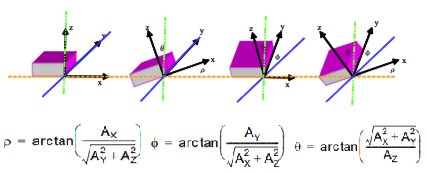
\includegraphics[scale=.95]{tilt.png}\end{center}
\begin{it}\begin{center}Fig. 16 - Tilt from accelerometer \end{center}\end{it}
However, all accelerometers are completely insensitive to rotations about the gravitational field vector and cannot be used to determine such a rotation. For this reason, a magnetometer is used to determine the tilt around the Z-axis by using the magnetic poles of the planet as a reference.
\newline
\newline
Two data sets emerged from the three sensors for each axis: rotation and tilt. Having all this data, the real-time rotation of the PCB can be determined by using a complementary filter which merges the two data sets. The model is only limited by the sensing capacity of the three devices described in the datasheets.
\newline
\newline
Finally, the barometer is used to determine the vertical position of the device by using the pressure to determine altitude. The data samples from this device drive the auto-level function of the pilot.
\newline
\newline
The passive components used by the three devices consist of capacitors for voltage noise filtering. One special arrangement required by the magnetometer (Figure 18 - 4) is magnetic insulation. That is, inside the perimeter of the chip no wire, copper layer or magnetic device is allowed because this would induce a magnetic field, thus altering the natural magnetic reference of Earth.
\subsection*{Writing programs to the board}
The reset pin has a very important function for the microcontroller. It is used by the external devices to reset the device when flashing the memory or when uploading a program and it can also be used by the user to reset the program running on the board. It is connected to both in-circuit serial programming (ICSP) interface (RST tag in Sheet 1/3 Appendix 1) and Data terminal ready (DTR) interface (DTR tag in sheet 1/3 Appendix 1).
\newline
\newline
The ICSP and DTR interfaces (Figure 18 - 9 and 10) have been joined together to minimize the number of pins necessary for the two. They share 3 pins (two ground pins and the 3.3V line). The ICSP interface is used for accessing the microcontroller's bootloader. The microcontrollers are shipped without any software installed, thus, when mounting it on a board for the first time, it is not possible to upload any software before the bootloader is burned. Burning the bootloader is done through the ICSP interface. The DTR interface, on the other hand, provided the bootloader has been burned, facilitates the upload of binary code to the flash memory (32KB).
\subsection*{Sending commands to the board}
The synchronous program running on the microcontroller is actively listening for a signal on the interrupt pin PD2 (D2 in short or INT0PCINT18 in Appendix 1). The interrupt has the task of detecting the rising edges of the PPM protocol. Together with the internal timer, the rising edge listener triggers a function which records the time interval between subsequent pulses. When the interval is longer than a threshold it assembles the received information, sends it to the main task and then it waits for the next rising edge. By repeating this process, the microcontroller can register and manipulate the analog signal generated by the Raspberry Pi.

\subsection*{Power distribution and power measurement}
The board, not only powers the components it houses, but it also delivers high power (12V at 15A) to the BLDC\footnote{Brushless Direct Current} motors. It is essential to separate the two voltage levels as the 3.3V lines powering the devices on the board are susceptible to noise (the noise could alter i2c devices and reference signal lines used by the microcontroller and sensors). Finally, heat dissipation precautions were necessary for designing the high current lines mentioned earlier. This aspect will be experimentally analyzed in the next section.
\newline
\newline
Distributing power to the components driving the logic on the drone, including the RaspberryPi, the microcontroller and the sensors, is done by using a feature offered by the ESCs (Electronic Speed Controllers). These receive 12V from the PCB to power the motors and can deliver up to 12W of power (5V at 3A) through the BEC (Battery Eliminator Circuit). The BEC line s shown in Figure 18 - 16. Of the three pins, the outer two are GROUND and 5V. This powers the 5V line which is used by three devices: The Raspberry Pi Zero, the i2c current sensor and the voltage regulator (Figure 18 - 7, IMU\_LDO). This then transforms the 5V level to 3.3V. The array of capacitors from its output filters the voltage from noise. The result is a clean 3.3V voltage level that can be used by the microcontroller, the three sensors and the i2c bus connecting them. Figure 17 shows the 5V (red) and 12V (blue) lines.
\begin{center}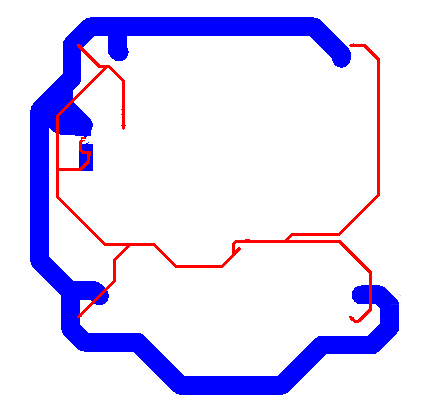
\includegraphics[scale=.35]{power_wires.png}\end{center}
\begin{it}\begin{center}Fig. 17 - Power lines in air \end{center}\end{it}
Finally, the power meter (Figure 18 - 5) uses a low, constant resistance resistor (Figure 18 - 12) to measure the current and voltage through the high current power line. As explained earlier, the output of this sensor is sent to the client application to derive the battery level.
\subsection*{Manufacturing and build}
Once the design was finished, the manufacturing files (Gerber) have been generated and sent to a PCB printing facility in Shenzen, China. After the initial prototype arrived, a second review was generated to correct some tolerance errors. The revision history can be found \hyperlink{https://easyeda.com/be.mihai22/project-hawk}{here}.
\clearpage
\pagebreak

\begin{figure*}
\begin{center}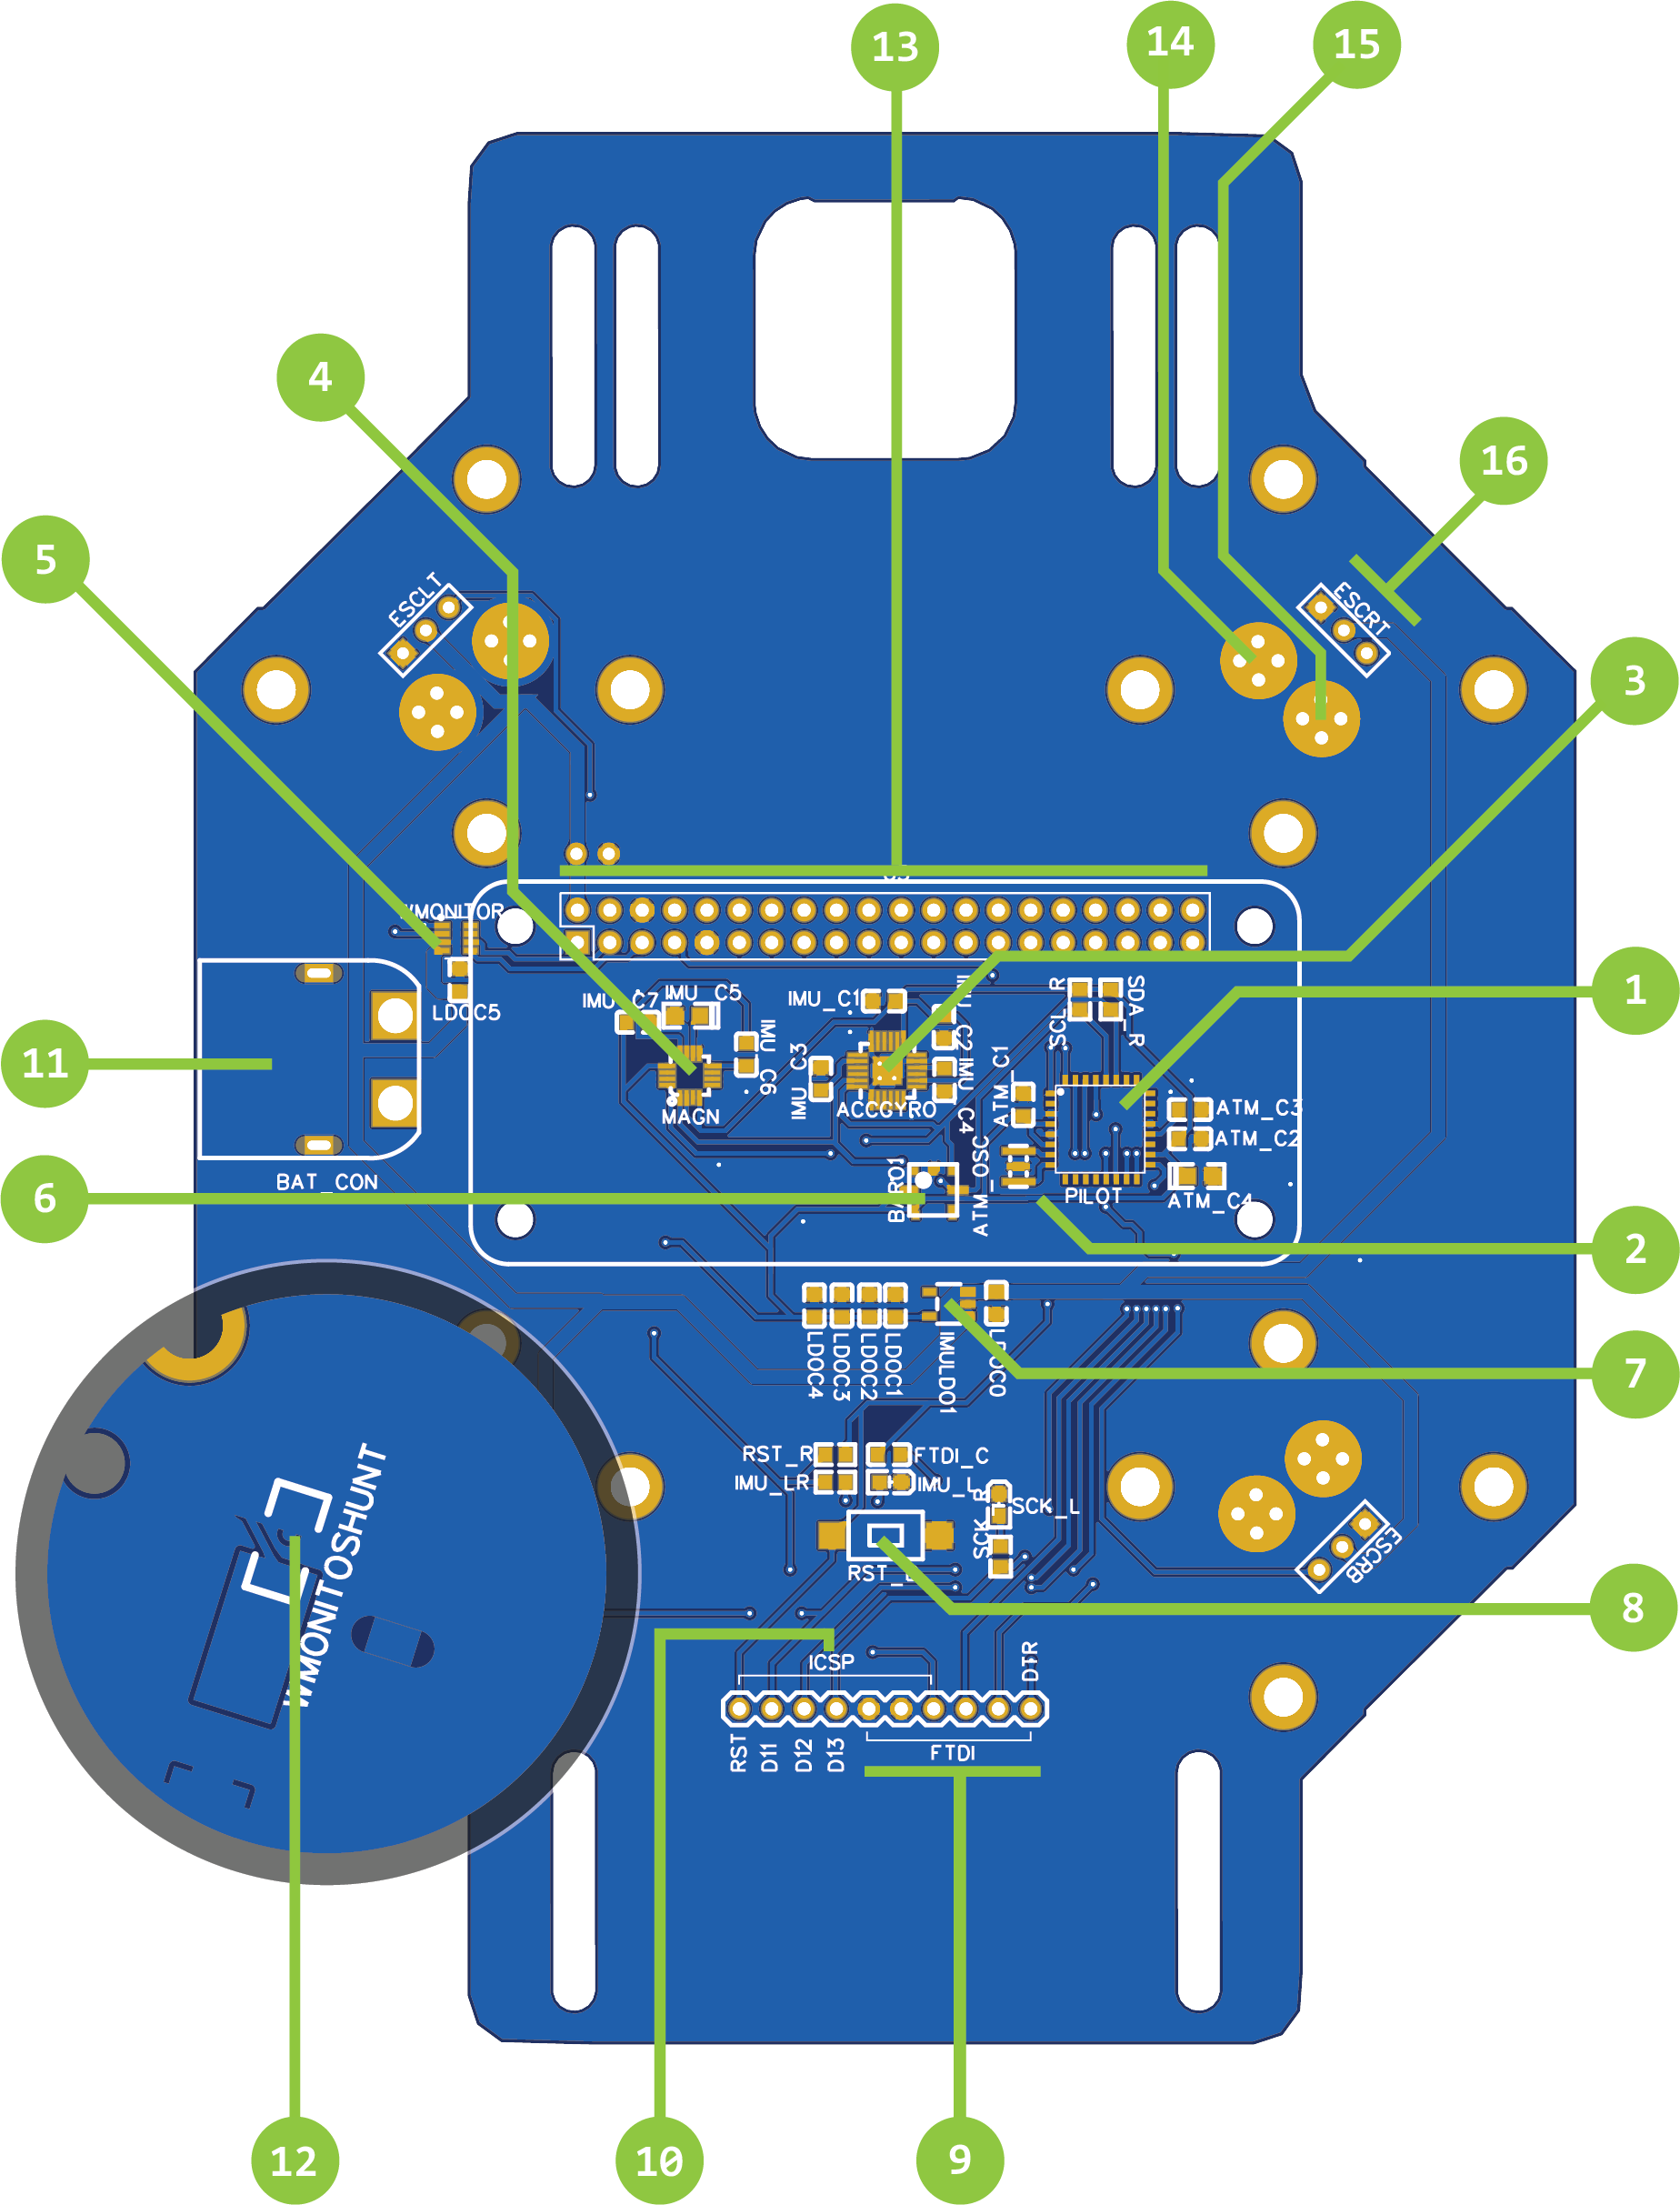
\includegraphics[scale=.95]{pcbschematic.png}\end{center}
\begin{it}\begin{center}Fig. 18 - Project HAWK PCB Schematic \end{center}\end{it}
\begin{multicols}{2}
\begin{itemize}
    \item[] 1. Atmel ATMega328P - 8 bit microcontroller
    \item[] 2. 16MHz quartz oscillator
    \item[] 3.  Accelerometer + Gyroscope - MPU6050 - 6 DOF
    \item[] 4. Magnetometer - HMC5833L - 3 DOF
    \item[] 5. Power meter - Texas Instruments INA219
    \item[] 6. Barometer - Bosch BMP180 
    \item[] 7. 5V to 3.3V voltage regulator
    \item[] 8. Reset button
    \item[] 9. FTDI Interface
    \item[] 10. ICSP Interface
    \item[] 11. Battery power connector - XT60 
    \item[] 12. 0.02 Ohm shunt resistor
    \item[] 13. Raspberry Pi 40 pin header
    \item[] 14. ESC Ground
    \item[] 15. ESC 12V
    \item[] 16. ESC BEC Ground (square), signal (middle), BEC 5V
\end{itemize}
\end{multicols}
\end{figure*}
\clearpage
\pagebreak
\section{Experimental evaluation}
In this project two features were tested: LTE connectivity stability and PCB temperature stability in high current delivery circuit.
\subsection{LTE latency experiment focusing on towers handover}
In order to prove LTE stability and availability, the following requirements had to be met:
\begin{itemize}
    \item Civil Aviation Authority flight conditions
    \item A public safe flight space
    \item An LTE mobile provider available in the area such that two or more towers will have borders within the safe flight space.
    \item Logging software to track key performance indicators (KPIs)
\end{itemize}
To fulfil the first condition, the drone was flown at 150 feet and the perimeter was closed for the duration of the test (approximately 25 minutes). The location was Birmingham, England - Selly Oak - Selly Park (52.438816, -1.924228) - which is covered by the three BT antennas showcased in Figure 19. Therefore, the sight fulfils the second and third conditions.
For this experiment, the towers will be named according to the zone they serve (e.g B serves zone B etc).
\begin{center}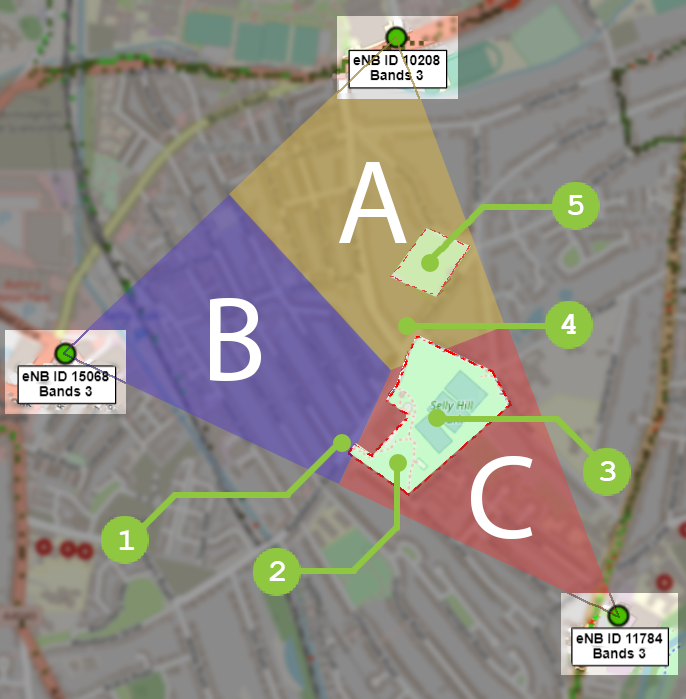
\includegraphics[scale=.60]{routersmap.png}\end{center}
\begin{it}\begin{center}Fig. 19 - Test Site - Selly Park and Elmdon Road Cricket Ground \end{center}\end{it}
A, B and C are the areas covered by the three towers (highlighted in green in Figure 19). This is a relative approximation based on entries found in the biggest open database for cell towers, called OpenCelliD \footnote{Please see the map without filtered providers \hyperlink{https://opencellid.org/#zoom=16&lat=52.44013&lon=-1.92437}{here}}. The information in the database was backed with on-terrain investigations for the coverage boundaries of the towers (i.e the accuracy for A, B, C borders was manually checked). Results indicated that the information in the database is accurate with a tolerance of 12 meters, resulting in an accuracy of 97\%.
\newline
\newline
To analyze the performance three aspects have been continuously observed\citep{maskey_2015_latency}:
\begin{itemize}
    \item The location of the drone
    \item The serving LTE radio cells
    \item LTE Network KPIs (DL/UL latency and RSRQ)
\end{itemize}
RSRQ is a quality indicator in LTE communication which takes into account two parameters: RSRP (Reference Signal Received Power) and RSSI(Reference Signal Strength Indicator). RSRP is at the type of measurement which takes into account the power of the LTE Reference Signal over the full bandwidth and narrowband. RSSI on the other hand measures only the average total received power for observed OFDM symbols (i.e orthogonal frequency-division multiplexing) over N resource blocks. Thus, RSRQ is derived using this formula: $RSRQ = (N * RSRP) / RSSI$.
\newline
\newline
The latency was recorded using \textbf{tcpdump}. Because packets are sent at a constant interval (4 ms), the latency sample will be the delta time of the RX packets - 4ms. This applies to both UL and DL. The RSRQ was sampled directly from the modem which has the reference signal RX quality (RSRQ) and reference signal RX power (RSRP) monitors built-in.
\begin{center}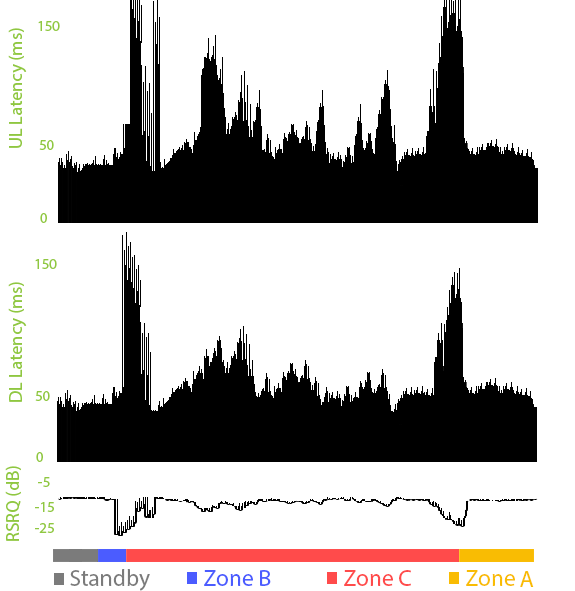
\includegraphics[scale=.85]{KPIs.png}\end{center}
\begin{it}\begin{center}Fig. 20 - KPIs in air \end{center}\end{it}
The drone travelled through locations 1, 2, 3, 4, 5 highlighted on the map in Figure 19 in this order. During this, DOWNLINK and UPLINK latency were recorded, as well as the RSRQ as seen in Figure 20.
The coloured bar represents the path from point 1 (zone B) to point 5 (zone A) through zone C. The flight speed of the drone was not taken into account when sampling the data, thus it appears that the drone spent more time in zone C.
\newline
\newline 
At the beginning of the test, the drone was standing by in zone B, receiving data packets from the client (the grey portion of the path). Then, the drone took off and it started travelling inside zone B for a short period when the handover was made from tower B to tower C. Looking at the graph, a spike in DL and UL latency can be observed. This is driven by the most important KPI, the RSRQ which also dips dramatically bellow -20dB. Next, during the flight in zone C, a direct relation between dips in RSRQ and latency can be observed. Last but not least, when the towers handed over the connection from tower C to tower A, another negative peak in RSRQ was recorded. Accordingly, the latency spikes too.
\newline
\newline
This test was also replicated on foot (pedestrian height) and the values recorded are shown in Figure 21.
\begin{center}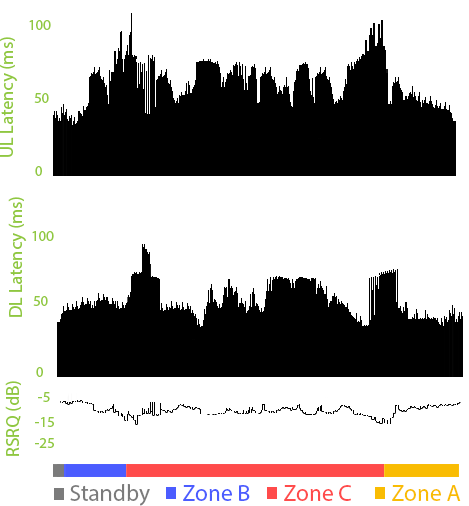
\includegraphics[scale=.90]{kpi_on_foot.png}\end{center}
\begin{it}\begin{center}Fig. 21 - Key performance indicators on foot \end{center}\end{it}
It can be observed that the spikes arising at handover are, on average, twice as high when the test was performed in the air compared to the test performed on foot. 
The disparity between the two results is explained by the fact that the LTE signal is optimized for general consumer use for cars, houses and pedestrians.
\newline
\newline
By comparing Figure 20 with Figure 21, two conclusions can be drawn from this experiment:
\begin{itemize}
    \item [a)] Handovers between towers generally introduce latency spikes in packet transmission
    \item [b)] The spikes at high altitude (40+ meters) are more severe
\end{itemize}
For statistical accuracy, the two tests have been performed seven times and the slight variation in trajectory and speed of the drone have been taken into account, normalizing the data by using a median filter and then cropping the stable segment.
In conclusion, this experiment reveals two of the limitations of the LTE network: tower handover and lack of optimization for drone flight space.
\subsection{PCB temperature variation experiment}
A good PCB design has to take into account not only the compatibility of the components that are mounted on the board but also whether the components are affected by changes in physical conditions. This experiment focuses on analysing whether the temperature on the board increases during a flight when the power through the board reaches peak values of 130W.
\newline
\newline
The experiment consists of analyzing the temperature variation and power dissipation on the board \citep{cheng_2008_theoretical}. Power dissipation is the power that is transformed to heat by resistors, including the metal conducting the current to components. Power dissipation can be derived from Ohm's Law $V = I * R$ where R is the resistance, V is the voltage and I is current; finding the current through the resistor then allows using the formula for power: $P = I * V$. Thus, $P = V^2*R$. The power dissipated through heat is directly proportional to the electric energy (which is linear to power $E = P * time$), but other factors influence whether the board stores the heat energy or not. Some of then are the thermal conductivity of the materials, ventilation and ambient temperature. Because of this, it is not facile to determine the heat dissipation model from theory, thus an experiment is necessary.
The data gathered for this experiment was collected from 3 sensors. Coincidentally, two of the i2c sensors that are used in stabilising the drone have thermometers integrated. The MPU6050 and the BMP180 temperature samples have been collected at a rate of 15 samples / second in a series of ten batches which were then averaged. In parallel, the power used by the system was monitored using the INA219 which runs over the Raspberry Pi i2c bus. The data is presented in Figure 22.
\begin{center}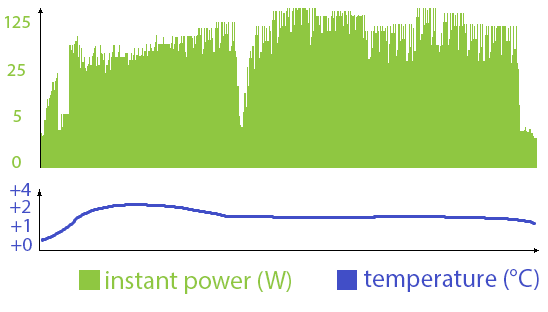
\includegraphics[scale=.70]{power_temperature.png}\end{center}
\begin{it}\begin{center}Fig. 22 - Heat/Power dissipation map \end{center}\end{it}
The drone follows a strict trajectory: It takes off vertically and continues straight up to 120 meters of altitude. After this, the motors stop and the drone is in a free fall. At 30 meters the motors are engaged again and the drone flies up to 80 meters of altitude again. In Figure 22 the green plot describes the instant power. The initial ramp describes the power-up of the motors and the later dip describes the free fall. In the end, the landing can be observed where the power dips again. During this, the temperature recorded has only risen by a 2.5$^{\circ}$C peak. As it can be observed in the blue graph in Figure 22, the temperature decreases once the drone reached a higher altitude. Three factors influenced the cooling in this case: 
\begin{itemize}
    \item the ambient temperature
    \item the decrease in temperature driven by an increase in altitude
    \item active cooling from the propellers
\end{itemize}
This experiment was conducted both for the first and second revisions of the PCB. In the first revision, the copper traces had a width of 2mm with a copper weight of 1oz\footnote{thickness is derived from weight / sqf}. The second revision has main power lines with a thickness of 5mm and a copper weight of 2oz. Because of this, the first revision was overheating past the point of melting the plastic in the arms of the drone.
In conclusion, this experiment proves the efficiency of wide high current power lines which pose less resistance to the flowing electrons.

\section{Improvements and Project Future}
This section describes the hardware and software improvements that could be implemented to resolve the disadvantages discovered during the experimental review regarding the LTE connectivity. What is more, this section addresses upgrades to make the flying machine even more versatile.
\subsection{LTE dual connection}
One potential solution to resolve the problem showcased in the experimental evaluation regarding tower handover is to use two active LTE connections from two different providers. To integrate the two modems, the protocol would have to be changed so that each packet is labelled with a sequence number. The packet is then sent through both connections at the same time and once it reaches the server a check is made to verify whether the packet has already been received through the other network path. If this is true, the packet is discarded. Otherwise, it means that the packet arrived first, thus providing the quickest route. In 80-90 per cent of the cases, the time gap between the packets with the same sequence number will be irrelevant in practice. During the handover, assuming that the signal towers from the two LTE internet providers differ in location, one packet will arrive faster through one of the modems that are not performing the handover, compared to the connection which is being switched from a tower to another. Thus, this would highly increase the reliability, the chance of double modem handover being very small \citep{nguyen_2018_how}
\subsection{Private LTE network}
Another solution to the problem mentioned earlier is deploying a private LTE network which could be optimized for altitude transmission. Compared to the consumer LTE broadband (which is designed for pedestrians, cars and home use), this network could satisfy the reliability to the level shown in the second part of the experiment (Figure 21) where the latency spikes during connection handover never exceeded 100 milliseconds \citep{amorim_2017_radio}. Nevertheless, the main drawback of this approach is the widespread infrastructure investment needed to support the technology.

\subsection{Low latency first-person view video streaming}
Given that the Broadcom BCM2835 which is powering the RaspberryPi Zero used for powering this project is marketed as a video-streaming-ready system on chip, it would be great to analyze the possibility of streaming live video with a latency under 150ms. One way to implement could be using gstreamer. Gstreamer is a media library oriented at high pace data delivery. To make this work additional configurations such as disabling the power limit the modem can draw from the board has to be made. 
\section{Conclusion}
This  report  has  outlined  the  main  advantages  and  dis-advantages  of  data  packet  communication  over  commercialLTE  networks  by  creating  a  new  platform  built  with  open-source  hardware  and  software.  Although  there  are  downsides  to  using  LTE  networks, the results of the experimental evaluation suggest that LTE is an efficient and reliable technology for drone piloting. moreover, rigorous studies could be conducted in areas with varied geographical features in order to test the limits of the LTE technology. The collection of large amounts of data will both increase the acuracy of the results and widen our hirozons in understanding what improvements to the LTE technology are most advantageous.\par
\clearpage
\newpage
\bibliographystyle{agsm}
\bibliography{citations}

\begin{figure*}
\section*{Appendix}
\begin{center}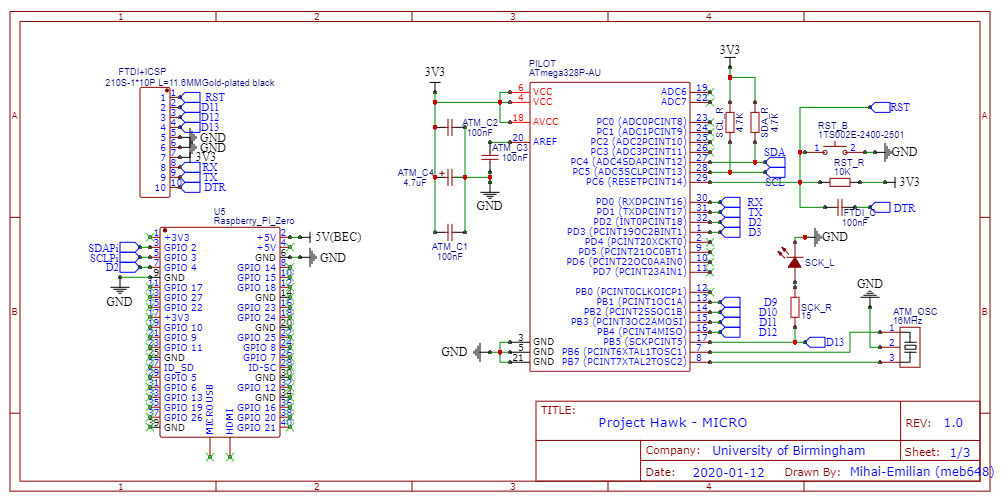
\includegraphics[scale=.5]{MICRO.png}\end{center}
\begin{it}\begin{center}Appendix 1 - Project HAWK MICRO Schematic \end{center}\end{it}

\begin{center}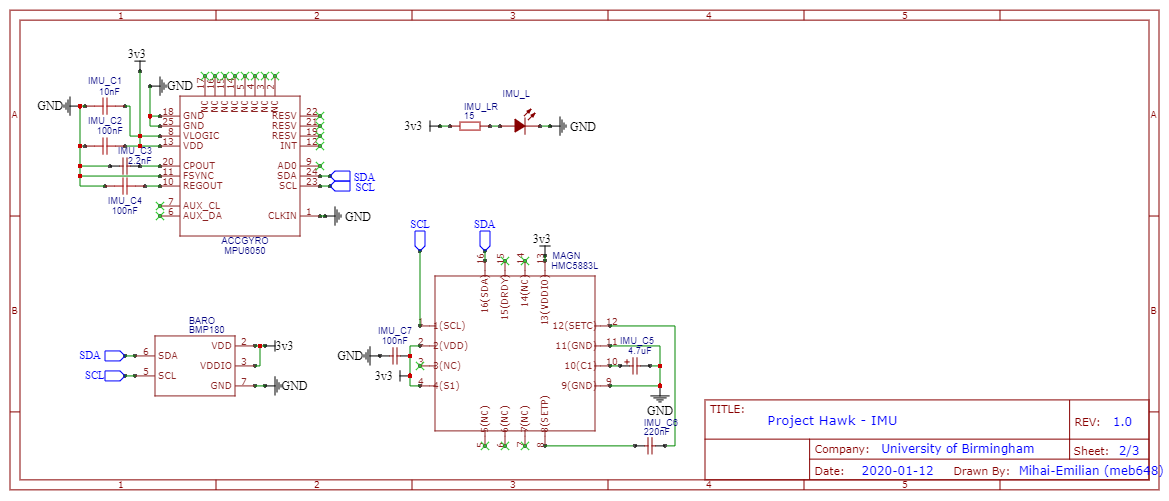
\includegraphics[scale=.428]{IMU.png}\end{center}
\begin{it}\begin{center}Appendix 2  - Project HAWK IMU Schematic \end{center}\end{it}
\end{figure*}
\clearpage
\begin{figure*}
\begin{center}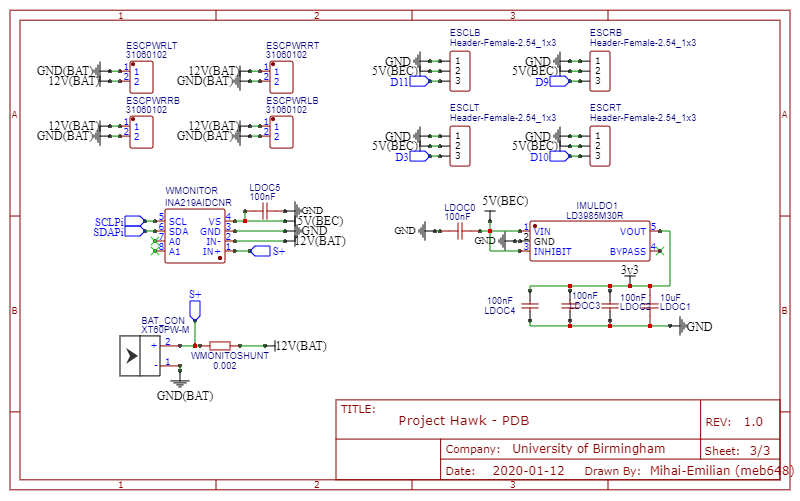
\includegraphics[scale=.65]{PDB.png}\end{center}
\begin{it}\begin{center}Appendix 3 - Project HAWK PDB Schematic \end{center}\end{it}
\end{figure*}
\clearpage
\end{document}
